\documentclass{tcc}

\begin{document}
\pagestyle{empty} %retira numeração da página
%Dados do TCC%
\author{Organización de Datos 75.06}
\title{Competencia de Machine Learning}
\newcommand{\subtitulo}{San Francisco Bay Area Biking}
\newcommand{\nomedocurso}{Organización de Datos 75.06}
\newcommand{\titulobar}{titulo}
\newcommand{\orientador}{Luis Argerich
\newcommand{\profa}{Nome do Professor A}
\newcommand{\profb}{Nome do Professor B}
\newcommand{\profc}{Nome do Professor C}
\newcommand{\insta}{Instituicao do Professor A}
\newcommand{\instb}{Instituicao do Professor B}
\newcommand{\instc}{Instituicao do Professor C}
\newcommand{\coordenador}{Nome do Coordenador}
\newcommand{\departamento}{Departamento de Computación}

\begin{center}
\LARGE{\bf INFORME TRABAJO PRÁCTICO 2}\\
\Large{\bf Competencia de Machine Learning}\\
\end{center}



\begin{figure}[H]
\centering
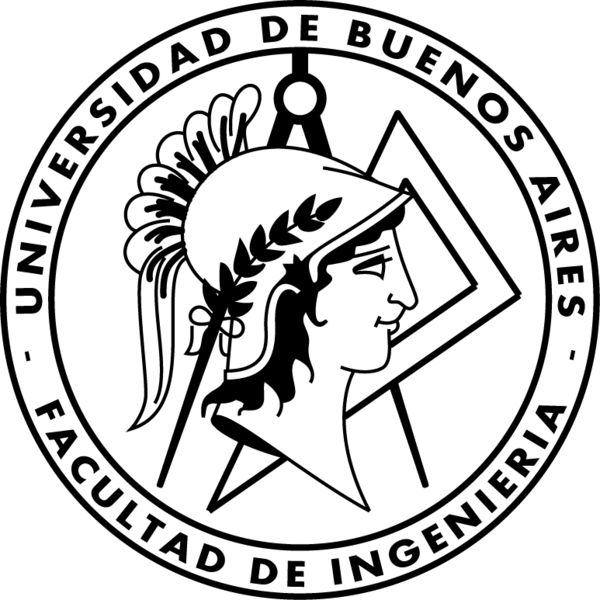
\includegraphics{imagenes/fiuba.png}
\end{figure}

\begin{center}
ORGANIZACIÓN DE DATOS - 75.06/95.58 \\
UNIVERSIDADE DE BUENOS AIRES

\end{center}

\vspace{1in}

\vspace{3em}

\begin{center}
Maximiliano, maxicc4@gmail.com\\
Prieto Pablo, prietopablo89@gmail.com\\
Galván Nahuel, nahuelgalvan@gmail.com\\
Prado María Florencia, 96626, pradomflorencia@gmail.com
\end{center}

\vfill
\begin{center}
Primer cuatrimestre, \the\year
\end{center}
\newpage
\begin{center}
\theauthor
\end{center}
\vspace{3in}
\begin{center}
\LARGE{\thetitle}\\
\end{center}

\vspace{2in}

\begin{flushright}
El propósito de esta competencia es predecir
la duración \\de viajes en bicicleta en la
Bahía de San Francisco \\en base al set de datos brindado por Kaggle
\\
\vspace{0.2in}



\end{flushright}

\vfill
\begin{center}
Primer cuatrimestre de \the\year
\end{center}


\newpage

%Resumo%
\section*{\centering{RESUMEN}}
Um resumo de trabalho de conclusão de curso é do tipo informativo e deve conter somente um parágrafo. A estrutura do resumo deve conter essencialmente os seguintes tópicos: apresentar inicialmente os objetivos do trabalho (o que foi feito?), a justificativa (porquê foi feito) e, finalmente, os resultados alcançados. O resumo deve informar ao leitor todas as informações importantes para o que o leitor possa entender o trabalho desenvolvido, quais foram as finalidades, a metodologia que o autor utilizou e os resultados obtidos. Deve conter frases curtas, porém completas (evitar estilo telegráfico); usar o tempo verbal no passado para os principais resultados e presente para comentários ou para salientar implicações significativas.  O resumo em português e inglês são obrigatórios e não devem passar de 200 palavras.

{\bf Palavras-chave:} $<$Primeira palavra$>$,  $<$segunda palavra$>$, $<$até 5 palavras$>$.
$<$ Obs.: as palavras-chave devem ser escolhidas com bastante rigor, pois devem representar adequadamente os principais temas abordados pela pesquisa.$>$





\newpage

%Sumário%
\renewcommand*\contentsname{Contenido}
\pagestyle{plain} %mostra numeração da página%
\tableofcontents

\newpage
\section{INTRODUCCIÓN}

\subsection{Definición del Problema}

La competencia se desarrolla en la plataforma de Kaggle, se provee un archivo "train.csv"que debe ser usado para entrenar un modelo de Machine Learning y un archivo "test.csv" que tiene los datos de los viajes a predecir. Adicionalmente pueden usarse los datos de las estaciones, del status de cada estación minuto a minuto y la información meteorológica.

\subsubsection{Objetivo general}
Con el análisis exploratorio realizado para el primer trabajo práctico más el estudio de diferentes algoritmos y perfeccionamiento de los mismos en base las características de nuestro set de datos pretendemos lograr un modelo que realice buenas predicciones.

\section{CONCEPTOS GENERALES}

\subsection{Machine Learning}
Conocemos como Machine Learning a la rama de la computación que estudia el diseño de algoritmos que son capaces de aprender. Este tipo de algoritmos son utilizados en la actualidad para muchas aplicaciones, por ejemplo para recomendaciones de películas o para ranquear sitios web en base a una consulta.


\subsection{Algoritmo y Modelo}

Se parte de un algoritmo de Machine Learning y se desea obtener lo que conocemos como modelo, aquel que se adapte mejor a nuestro set de datos. El algoritmo es el enfoque general que se toma. El modelo es lo que se obtiene cuando se ejecuta el algoritmo sobre el set datos de entrenamiento y lo que se usa para hacer predicciones sobre nuevos datos. Se puede generar un nuevo modelo con el mismo algoritmo pero con datos diferentes, o un modelo diferente de los mismos datos con un algoritmo diferente. 
Cada modelo tiene un conjunto de parámetros e hiper-parámetros que necesita para funcionar. Los parámetros los descubre el algoritmo a partir de los datos, los hiper-parámetros, en cambio, son datos que debemos pasarle al algoritmo para funcionar\footnote{Apunte del curso, 11.1
Evaluación de Algoritmos de ML}. Por lo tanto la clave está en encontrar los hiper-parámetros óptimos.

\subsection{Cross Validation}

El proceso de K-fold Cross Validation comienza particionando el set de entrenamiento en k bloques, luego vamos a realizar varias iteraciones en las cuales entrenamos nuestro algoritmo con k 1 bloques y lo validamos con el restante \footnote{Apunte del curso,11.1.1
Cross Validation}.

\begin{figure}[h]
\centering
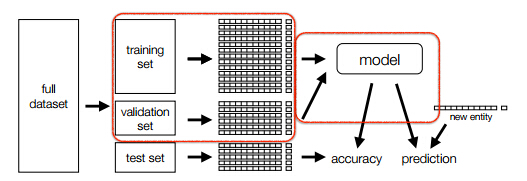
\includegraphics[height=4.5cm]{imagenes/crossValidation}
\caption{Cross Validation esquema}
\label{fig:exemplo}
\end{figure}

Este método será utilizado a en el desarrollo de este trabajo práctico. Más adelante explicaremos el porqué usarlo y los beneficios que trae.


\section{METODOLOGÍA}

\subsection{Definición del Problema}


\subsection{Preparación de los Datos}
Antes de comenzar la construcción de cualquier modelo es fundamental realizar esta etapa. La preparación de los datos es difícil, debemos definir cuál es la mejor forma de manejarlos para describir el problema.

Wickham señala que no es un proceso de una sola vez, que es iterativo como entender el problema más profundo en cada paso sucesivo. El objetivo es estructurar los datos para facilitar el análisis de datos.\cite{RforDataScience}



\begin{itemize}
   \item Eliminamos la columna de start\_station\_name y dejamos start\_station\_id.
    
    \item Eliminamos la columna de end\_station\_name y dejamos start\_station\_id.
    
    \item En subscription\_type tenemos dos posibles valores, 
    subcriber o customer el primero será 1 y el segundo 2.
    
    \item
    
\end{itemize}

Utilizaremos una técnica simple en la que sustituimos cada valor faltante por la mediana de todos los valores presentes.

\subsection{Estudio de Posibles Algoritmos}

Como lo demuestra el "No Free Luch Theorem" no existe un mejor algoritmo para cada categoría de problemas en Machine Learning.  Por eso es que vamos a estudiar varios y decidir cuál, o la combinación de cuáles nos brinda un mejor modelo para predecir un nuevo evento siguiendo el set de datos de la competencia.
Comenzaremos con algoritmos simples y de a poco intentremos refinarlos.

\subsection{Construcción de Algoritmos}

\subsection{Interpretación de Resultados}

\subsection{Evaluación de Algoritmos}

\subsection{Mejoramiento de Resultados}

A good heuristic is to keep increasing the number of models until performance levels off.

Also, it is generally a good idea to have sample sizes equal to the training data size.


\subsubsection{Ensamblado de Algoritmos}

\subsection{Presentación de Resultados}

\subsection{Sckit-Learn}

En nuestra búsqueda de información y recomendaciones para el desarrollo de nuestro modelo encontramos Sckit learn, una librería para Python. 
En la documentación figura una diagrama que nos guía para encontrar posibles estimadores para nuestro problema.

http://scikit-learn.org/stable/modules/tree.html#tree !!!

http://www.dummies.com/programming/big-data/data-science/how-to-create-classification-and-regression-trees-in-python-for-data-science/

https://cambridgespark.com/content/tutorials/getting-started-with-regression-and-decision-trees/index.html

https://gist.github.com/JustGlowing/9093f9f72f68b2ede79a

https://dominicbreuker.com/boston_housing/

\begin{figure}[h]
\centering
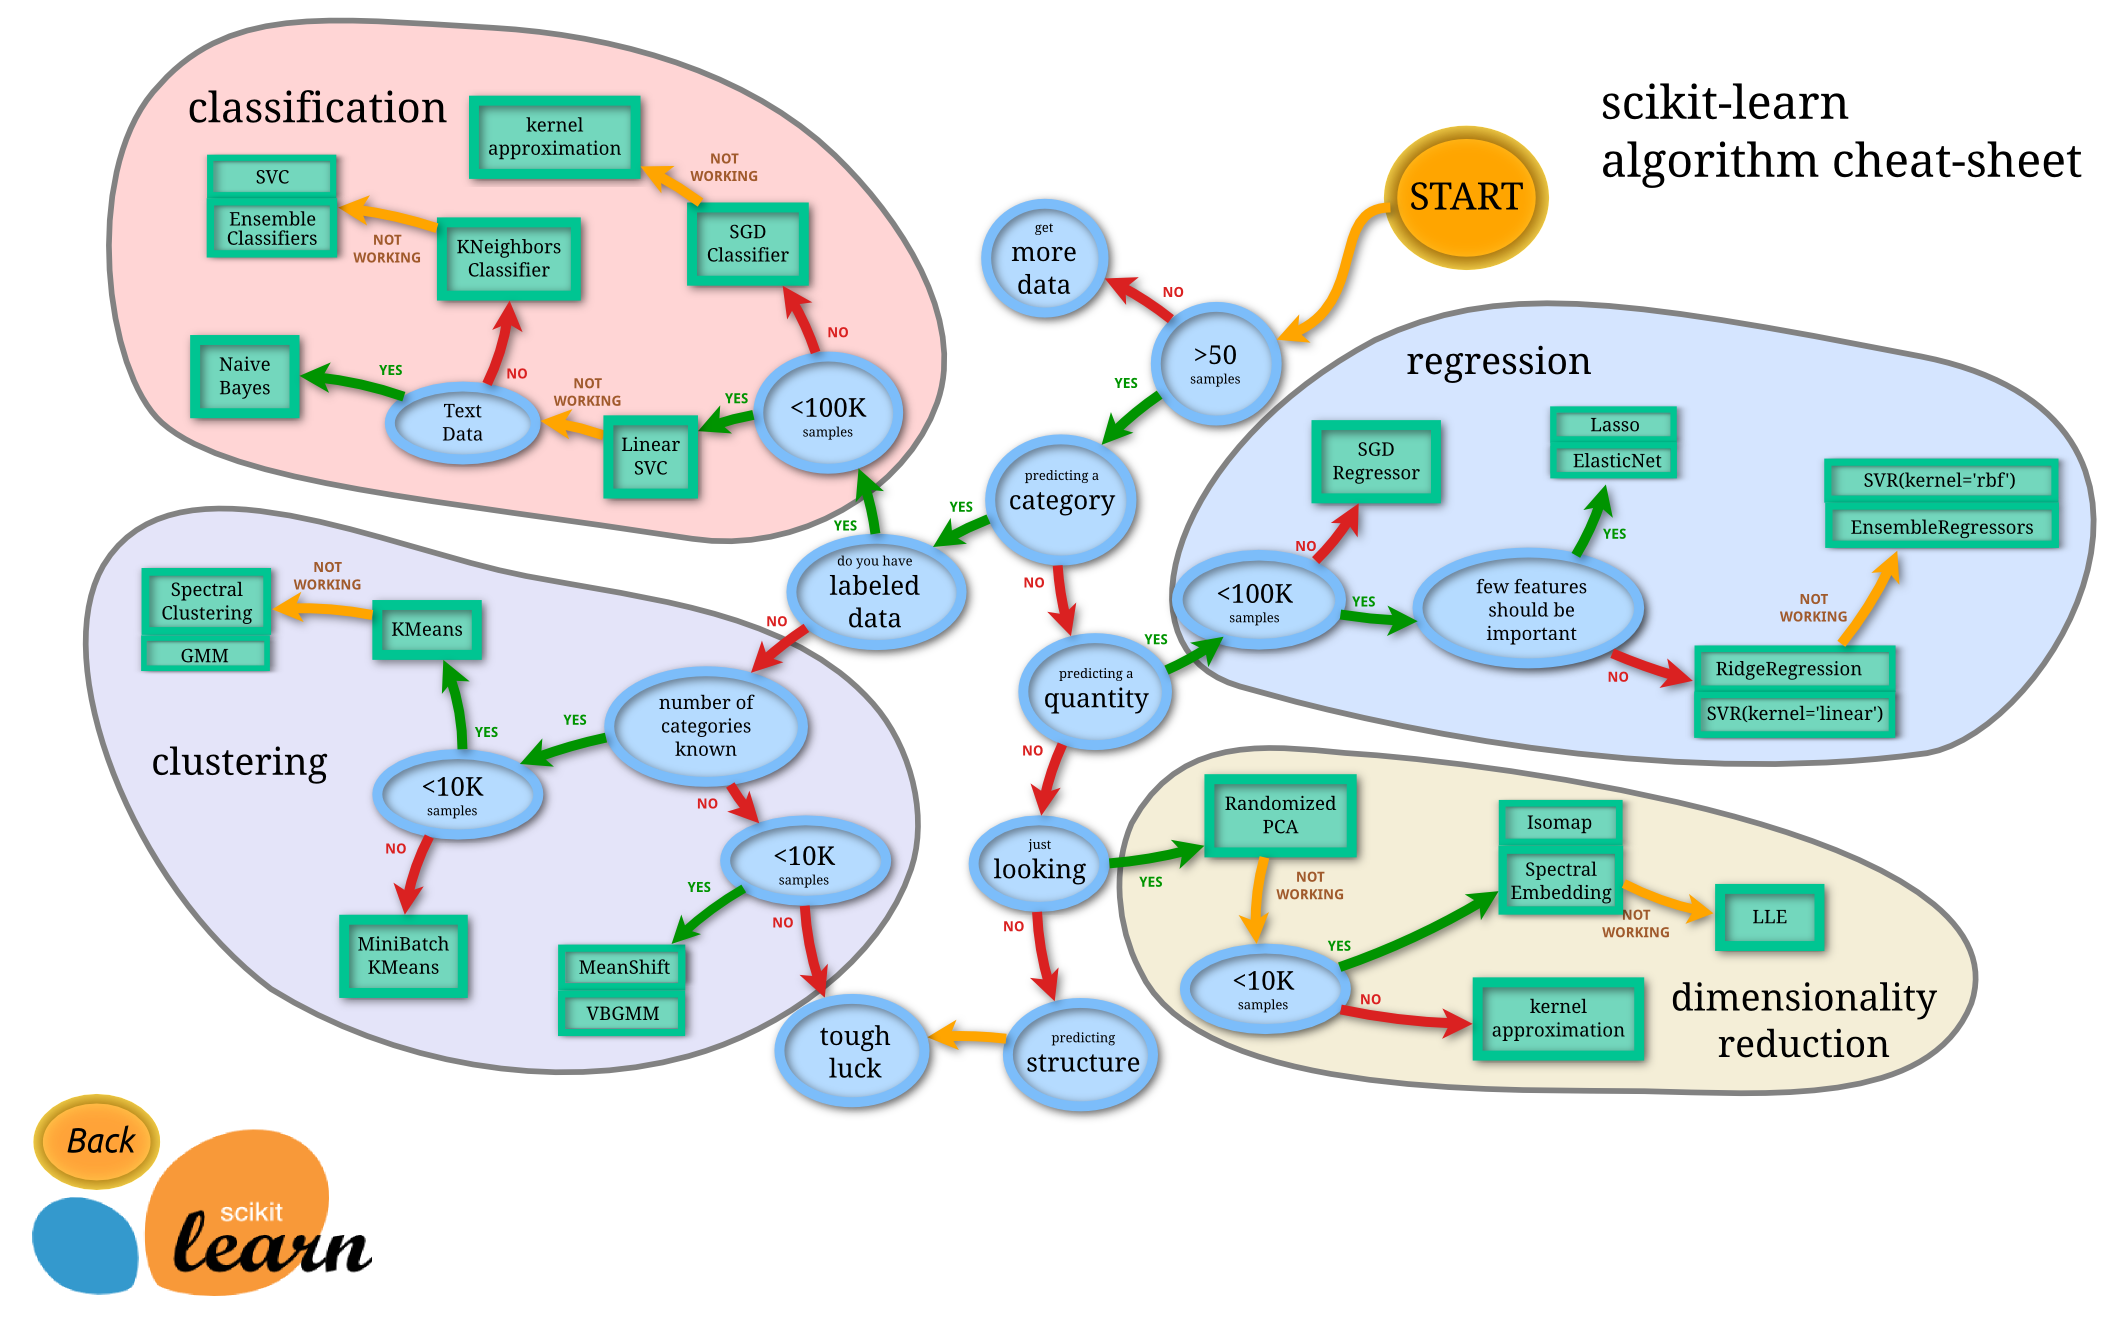
\includegraphics[height=10cm]{imagenes/sckit.png}
\label{fig:exemplo}
\end{figure}

\subsection{SGD Regresor}
Dado a que tenemos una cantidad de datos mucho mayor a 100k probaremos con SGD Regresor


\begin{table}[h]
\centering
\caption{ Modelo de como as tabelas devem ser inseridas no texto }
\vspace{0.2in}
\newcolumntype{C}{>{\centering\arraybackslash}X}%
\newcommand{\rowstyle}[1]{%
  \protected\gdef\currentrowstyle{#1}%
}
\begin{tabularx}{\textwidth}{>{\bf}C|C|C|C}
\hline 
\textbf {Índice} & \textbf{Coluna 01} &\textbf{ Coluna 02} & \textbf{Coluna 03} \\ \hline \hline
Linha 01 & & & \\ \hline
Linha 02 & & & \\ \hline                         

\end{tabularx}
\end{table}






\begin{table}[h]
\centering
\caption{ Modelo de como as tabelas devem ser inseridas no texto }
\vspace{0.2in}
\newcolumntype{C}{>{\centering\arraybackslash}X}%
\newcommand{\rowstyle}[1]{%
  \protected\gdef\currentrowstyle{#1}%
}
\begin{tabularx}{\textwidth}{>{\bf}C|C|C|C}
\hline 
\textbf {Índice} & \textbf{Coluna 01} &\textbf{ Coluna 02} & \textbf{Coluna 03} \\ \hline \hline
Linha 01 & & & \\ \hline
Linha 02 & & & \\ \hline                         

\end{tabularx}
\end{table}
\section{ANÁLISIS DE RESULTADOS}
Toda pesquisa deve apresentar uma análise sobre a investigação que foi realizada através da metodologia que foi aplicada. Nesta sessão é interessante inserir tabelas, gráficos, imagens que mostrem os resultados, análise de dados coletados, etc.

É interessante que nessa sessão o autor compare os seus resultados com os resultados de outros trabalhos existentes. Essa comparação aumenta a qualidade do trabalho e demonstra a relevância do mesmo. 

Nesta sessão o autor pode/deve incluir as contribuições científicas desenvolvidas tais como artigos, patentes, livros e outras contibuições que foram publicadas ou estão em fase de publicação e que são parte do trabalho.
\section{CONCLUSIONES}
An interesting difference between regression and classification is that the
correlation increases quite slowly as the number of features used increases. The
major effect is the decrease in PE*( tree). Therefore, a relatively large number of
features are required to reduce PE*(tree) and get near optimal test-set error.
The results shown in Table 6 are mixed. Random forest-random features is
always better than bagging. In data sets for which adaptive bagging gives sharp
decreases in error, the decreases produced by forests are not as pronounced. In
data sets in which adaptive bagging gives no improvements over bagging,
forests produce improvements.


Random forests are an effective tool in prediction. Because of the Law of Large
Numbers they do not overfit. Injecting the right kind of randomness makes
them accurate classifiers and regressors. Furthermore, the framework in terms
of strength of the individual predictors and their correlations gives insight into
the ability of the random forest to predict. Using out-of-bag estimation makes
concrete the otherwise theoretical values of strength and correlation.
For a while, the conventional thinking was that forests could not compete with
arcing type algorithms in terms of accuracy. Our results dispel this belief, but
lead to interesting questions. Boosting and arcing algorithms have the ability to
reduce bias as well as variance (Schapire et al [1998]). The adaptive bagging
algorithm in regression (Breiman [1999]) was designed to reduce bias and
operates effectively in classification as well as in regression. But, like arcing, it
also changes the training set as it progresses.
Forests give results competitive with boosting and adaptive bagging, yet do not
progressively change the training set. Their accuracy indicates that they act to
reduce bias. The mechanism for this is not obvious. Random forests may also
be viewed as a Bayesian procedure. Although I doubt that this is a fruitful line
of exploration, if it could explain the bias reduction, I might become more of a
Bayesian.
Random inputs and random features produce good results in classification--less
so in regression. The only types of randomness used in this study is bagging and
random features. It may well be that other types of injected randomness give
better results. For instance, one of the referees has suggested use of random
Boolean combinations of feature
%%%%%%%%%%%%%%%%%%%%%%%%%%%%% Referências %%%%%%%%%%%%%%%%%%%%%%%%%%%%%
\renewcommand{\refname}{\centering REFERENCIAS} %Centraliza nome Referencias%
\addcontentsline{toc}{section}{REFERENCIAS} %adiciona referencias ao sumario

\nocite{*}
\bibliographystyle{plain}
\bibliography{references}

%%%%%%%%%%%%%%%%%%%%%%%%%%%%%%%%%%%%%%%%%%%%%%%%%%%%%%%%%%%%%%%%%%%%%%%

%%%%%%%%%%%%%%%%%%%%%%%%%%%%% ANEXO %%%%%%%%%%%%%%%%%%%%%%%%%%%%%
\section*{\centering{A – ANEXOS Y APÉNDICES 1}}
\addcontentsline{toc}{section}{A - ANEXOS Y APÉNDICES 1}

Anexos e apêndices são materiais adicionais, utilizados para complementar o texto, acrescentados ao final do trabalho, com a finalidade de esclarecimento ou de comprovação.

Apêndices são elaborados pelo autor e visam complementar uma argumentação. Os Anexos não são elaborados diretamente pelo autor e servem de fundamentação teórica, comprovação e ilustração (ex. mapas, leis, estatutos entre outros). Os apêndices devem aparecer antes dos anexos.

\end{document}